\section{Background}

Monitor automata are defined as the quintuple $(\sum, S, s_0, \delta, F)$ where $\sum$ is the input alphabet, $S$ is a finite non-empty set of states, $s_0$ is an element of $S$ and initial state, $\delta$ is the state-transition function $\delta: S \times \sum \rightarrow S$ and $F$ is the possibly empty set of final states and a subset of $S$.

\newpar Monitor automata operate on the set of possible effects of a statement in the Control-flow Graph which is defined as $E = \{$\texttt{alloc}, \texttt{free}, \texttt{read}, \texttt{write}, \texttt{uninit}, \texttt{call}, \texttt{lock}, \texttt{unlock}$\}$ by Abal \cite{EffectiveBugFinding}. 

\subsection{Double-unlock monitor automata}

A double-unlock monitor automata is defined as the quintuple $(\sum, S, s_0, \delta, F)$ where: 

\begin{itemize}
    \item $\sum = \{\texttt{unlock}, \texttt{lock}\}$, a subset of $E$
    \item $S = \{ locked_\rho, unlocked_\rho, error_\rho \}$, bound to a region $\rho$
    \item $s_0 = unlocked_\rho$ 
    \item $\delta =$ the relation $\{(locked_\rho, \texttt{unlock}_\rho, unlocked_\rho), (locked_\rho, \texttt{lock}_\rho, locked_\rho), \\
        (unlocked_\rho, \texttt{lock}_\rho, locked_\rho), (unlocked_\rho, \texttt{unlock}_\rho, error_\rho)\}$ 
    \item $F = error_\rho$  
\end{itemize}

An illustration of this monitor automata can be seen in figure \ref{double-unlock-automata}. 

\begin{figure}[H]
    \centering
    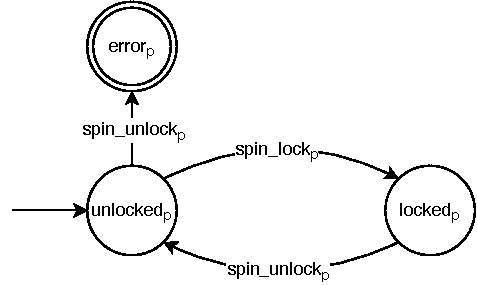
\includegraphics[width=0.5\textwidth]{background/figures/double-unlock}
    \caption{An illustration of a double-unlock monitor automata.}
    \label{double-unlock-automata}
\end{figure}
    
